\documentclass[12pt]{report}
\usepackage[utf8]{inputenc}
\usepackage[french]{babel}
\usepackage[T1]{fontenc}
\usepackage{xcolor}
\usepackage{listings}
\usepackage{graphicx}
\usepackage{titlesec}
\renewcommand{\thechapter}{}
\renewcommand*\thesection{\arabic{section}}
\setcounter{chapter}{1}
\setlength{\parindent}{0pt}
\addto\captionsfrench{
\renewcommand\chaptername{}}
\titleformat{\chapter}[display]
{\normalfont\huge\bfseries}{\chaptertitlename\ \thechapter}{20pt}{\Huge}
\titlespacing*{\chapter}{0pt}{-100pt}{40pt}
\title{Rapport de projet NachOS}
\author{
\'Equipe H\\\\
Mohd Thaqif ABDULLAH HASIM\\
Florian BARROIS\\
Cédric GARCIA\\
Hosseim NAHAL\\
Peio RIGAUX\\
}

\begin{document}
\maketitle


\chapter{Présentation de DesperadOS}

DesperadOS est un système d'exploitation basé sur le fonctionnement du système Unix. Il propose ainsi une version simplifiée des fonctionnalités de ce dernier, à savoir :
\begin{itemize}\renewcommand{\labelitemi}{$\bullet$}
\item Un système synchronisé d'entrées/sorties;
\item La gestion de plusieurs processus utilisateurs multithreadés.
\item Un système de fichiers permettant la manipulation de fichiers et la navigation à travers les répertoires et dont la taille des fichiers peut atteindre 112,5Ko.
\item La possibilité de communiquer en réseau.

\end{itemize}


\chapter{Spécifications}
\section{Entrées/Sorties}
\bigskip
\textbf{char GetChar():}

Retourne le caractère lu sur l'entrée standard.\\

\bigskip
\textbf{void PutChar(char c):}

Écrit le caractère \textit{c} sur la sortie standard.\\


\bigskip
\textbf{void GetString(char* buf, int n):}
 
Récupère \textit{n} caractères à partir de l'entrée standard. Cette récupération peut-être interrompue par '\textbackslash n',
auquel cas seuls les caractères avant le '\textbackslash n' sont pris en compte dans le tampon d'arrivée.
Si le nombre de caractères demandé est inférieur au nombre de caractères dans l'entrée standard, les caractères
restants sont mis en attente dans le tampon d'entrée. Ils seront récupérés lors du prochain appel à GetString().
Si le premier caractère présent dans le tampon d'entrée est '\textbackslash n', il est ignoré.


\bigskip
\textbf{void PutString(const char s*):}

Parcourt la chaîne de caractères \textit{n} et écrit caractère par caractère sur la
sortie standard jusqu'à la rencontre du caractère `\textbackslash 0' ou jusqu'à
ce que MAX\_STRING\_SIZE soit atteinte.


\bigskip
\textbf{void GetInt(int* n):}

Lit un entier depuis l'entrée standard. La limite est fixée à 16 caractères. Si la valeur n'est pas comprise dans l'intervalle [$-2^{31}$;
$2^{31}-1$],  elle prend la valeur de la borne la plus proche de cet intervalle. Si l'utilisateur entre uniquement le signe `-', le nombre stocké est zéro.
\bigskip

\textbf{void PutInt(int n):}

Affiche l'entier \textit{n} sur la sortie standard.\\


\section{Threads, processus et synchronisation}
\bigskip

\textbf{int UserThreadCreate(int f, int arg):}

Initialise un thread utilisateur qui appelle la fonction \textit{f} avec l'argument \textit{arg}. Bien que UserThreadCreate autorise un seul argument pour la fonction \textit{f}, il est possible de lui transmettre plusieurs arguments en les définissant comme paramètres d'une structure.
Retourne l’identifiant du thread créé.
\bigskip

\textbf{void UserThreadJoin(int tid):}

Interrompt l'exécution du thread appelant jusqu'à la terminaison du thread identifié par \textit{tid}.
\bigskip


\textbf{void UserThreadExit():}

Termine l'exécution du thread appelant. L'appel à UserThreadExit est facultatif puisqu'il est systématiquement réalisé lorsqu'un thread a terminé l'exécution de la fonction qui lui a été attribuée. Il peut néanmoins être utilisé pour forcer l'arrêt du thread avant la fin de sa tâche.
\bigskip


\textbf{void Sem\_init(Semaphore* sem, int val):}

Initialise la valeur du sémaphore \textit{sem} à \textit{val}.
\bigskip	


\textbf{void Sem\_wait(Semaphore sem):}

Décrémente la valeur du sémaphore \textit{sem}. Sem\_wait est bloquant tant que la valeur de sem est égale à zéro, empêchant ainsi la décrémentation.
L'appel à Sem\_wait nécessite que le sémaphore \textit{sem} ait été initialisé avec la fonction Sem\_init.
\bigskip


\textbf{void Sem\_post(Semaphore sem):}

Incrémente la valeur du sémaphore \textit{sem}. Si, une fois incrémentée, la valeur de \textit{sem} vaut 1 alors qu'un fil d'exécution est bloqué par Sem\_wait sur le même sémaphore \textit{sem}, alors ce fil d'exécution reprend son activité.
L'appel à Sem\_post nécessite que le sémaphore \textit{sem} ait été initialisé avec la fonction Sem\_init.
\bigskip


\textbf{void Sem\_destroy(Semaphore sem):}

Détruit le sémaphore \textit{sem}. Si \textit{sem} est détruit alors que des fils d'exécution ont été suspendus par un appel à Sem\_wait sur ce même sémaphore \textit{sem}, le comportement du système est indéterminé.
\bigskip


\textbf{void ForkExec(char* filename):}

Crée un nouveau processus qui exécute le programme passé en paramètre. \'A sa création, le nouveau processus contient un seul fil d'exécution. Les valeurs des registres de ce fil d'exécution sont identiques à celles des registres du fil d'exécution qui a appelé ForkExec.
\bigskip


\section{Système de fichiers}

Les commandes du système de fichiers doivent être exécutées de la manière suivante :
\textit{./nachos-filesys command}\\

Options disponibles :\\
\begin{itemize}\renewcommand{\labelitemi}{$\bullet$}
\item -l  : Liste le contenu du répertoire courant (équivalent de ls sur Unix).
\item  -D  : Affiche le contenu du disque et les blocs occupés utilisés par chaque fichier.
\item  -cp (nom1) (nom2) : Copie le fichier de nom \textit{nom1} dans le système de fichiers Nachos, sous le nom \textit{nom2}.
\item  -p (nom) : Affiche le contenu du fichier \textit{nom}. Échoue si le fichier n'existe pas.
\item  -md (nom) : Crée un répertoire de nom \textit{nom}. Échoue si le répertoire existe déjà ou si l'espace disque est insuffisant.
\item  -rd (nom) : Supprime le répertoire de nom \textit{nom}. Échoue si le répertoire n'existe pas, n'est pas vide, ou s'il s'agit du répertoire . ou ..
\item -cd (nom) : Déplace l'utilisateur sur le répertoire de nom \textit{nom} qui devient le répertoire courant. Fonctionne avec un chemin relatif. Échoue si le répertoire n'existe pas.
\end{itemize}

\bigskip
Pour la création de fichiers, la taille maximale autorisée est de 112,5Ko.


\chapter{Implémentation}

\section{Travail réalisé}
\bigskip

\subsection{Entrées/Sorties}

\textbf{char GetChar():} 

Utilise une version synchronisée de console->PutChar(const char ch)
afin de récupérer un caractère à partir de l'entrée standard.

\bigskip

\textbf{void PutChar(char c):} 

Utilise une version synchronisée de console->PutChar(const char ch)
afin d'afficher le caractère \textit{c} sur la sortie standard.
\bigskip


\textbf{void GetString(char * buf, int n):} 

Effectue \textit{n} appels à GetChar afin de remplir un tampon de caractères.
À chaque itération, des conditions permettent d'ignorer le caractère courant si
il correspond à EOF ou '\textbackslash n'.

\bigskip

\textbf{void PutString(const char s*):}

Parcourt la chaîne de caractères \textit{s} à l'aide d'une boucle et appelle PutChar avec chaque caractère.
\bigskip	
	

\textbf{void GetInt(int* n):}	
	
Récupère les caractères entrés un par un puis vérifie que le nombre demandé ne dépasse pas la taille d'un entier.
La chaîne de caractères résultante est convertie en entier.
\bigskip

\textbf{void PutInt(int n):}

Convertit \textit{n} en chaîne de 15 caractères avant de l'afficher sur la sortie standard.
\newpage	


\subsection{Threads, processus}

Un thread contient des champs entiers TID et BID.

Le BID correspond à l'indice du BitMap auquel le thread est référencé. Il est propre à l'espace d'adressage. Plusieurs threads peuvent donc posséder la même valeur de BID s'ils ne font pas partie du même processus. La gestion des threads est ainsi effectuée grâce au TID qui lui est unique dans le système. \\

Le nombre maximal de threads par espace d'adressage a été fixé à 16 car cette valeur nous a semblé suffisante pour une utilisation nominale du système par l'utilisateur et pour vérifier le bon fonctionnement du multithreading au sein du système.

\bigskip

L'implémentation des processus est différente de celle d'Unix. Dans DesperadOS, il n'existe pas de "lien de parenté" entre les processus. En conséquence, par exemple, un processus p2 créé suite à un ForkExec effectué par un thread d'un processus p1 peut appeler UserThreadJoin sur p1 et attendre qu'il termine, pour ensuite continuer son exécution normalement.
\bigskip

La pile est gérée de la manière suivante :
un objet BitMap est utilisé pour déterminer le secteur de la pile lié au nouveau thread et définir le numéro BID de ce thread.
\bigskip

Un type Semaphore a été défini pour procéder à l'implémentation des sémaphores utilisateur. 
La gestion du UserThreadJoin a été réalisée grâce à l'utilisation d'une liste chainée contenant un couple <TID,Semaphore>.
\bigskip

Enfin, un nouvel argument pointant sur la fonction UserThreadExit a été ajouté dans le fichier start.S lors de l'appel à UserThreadCreate. Ceci permet ainsi la terminaison automatique des threads lorsque ceux-ci ont terminé la tâche qui leur a été assignée.



\subsection{Pagination}


Notre stratégie d’allocation des pages physiques consiste en un tirage aléatoire via la méthode « GetEmptyFrame » . Un BitMap est utilisé pour vérifier si la frame est déjà allouée ou non.
\bigskip

La fin des processus et des threads est gérée automatiquement via un compteur pour déterminer s'il est nécessaire d'effectuer une interruption machine ou une terminaison de thread.
\bigskip


\subsection{Système de fichiers}

\bigskip
Pour permettre la création de répertoires, il a fallu distinguer les répertoires des fichiers "normaux". Ainsi dans la classe DirectoryEntry (qui représente une entrée de répertoire, quelle qu'elle soit) on ajoute un champ "isFile" de type booléen. Un booléen a été ajouté en paramètre des fonctions Find, Add et Remove de la classe Directory qui sont notamment utilisées lors de la création et suppression de fichiers ou de répertoires.
De plus, un répertoire racine, ne contenant qu'une entrée spéciale "." doit être créé, et défini comme répertoire courant au formatage.
\bigskip


\textbf{bool MakeDir(const char *name):} de la même manière que pour la fonction Create, cette fonction prend une chaîne \textit{name} en paramètre. On charge le répertoire courant à partir du secteur DirectorySector (constante fixée à 1) dans un objet de type Directory. Un test a été mis en place afin de  s'assurer qu'un répertoire de nom \textit{name} n'existe pas déjà (auquel cas la fonction renvoie false). On charge également le BitMap qui nous donne un secteur de données disponible (s'il n'y en a pas, la fonction renvoie false également). 
Un nouveau répertoire est créé. Il contient deux entrées spéciales (. et ..) et le FileHeader associé, qui est écrit sur le secteur libre défini précédemment. Enfin sur le répertoire courant une nouvelle entrée qui redirige vers ce secteur est ajoutée, et toutes ces modifications sont réécrites sur le disque.
\bigskip


\textbf{bool ChangeDir(const char *name):} Cette fonction va chercher le répertoire dont le nom (ou le chemin relatif) est passé en paramètre et, s'il existe, elle en fait une copie sur le répertoire courant situé sur le secteur DirectorySector numéro 1.
\bigskip


\textbf{bool RemoveDir(const char *name):} Si le répertoire dont le nom est passé en paramètre se trouve sur le répertoire courant (sauf . et ..), on vérifie si le répertoire est vide et, le cas échéant, on libère tous les secteurs qu'il utilise et le supprime des entrées du répertoire courant, puis on valide les modifications en réécrivant le répertoire courant sur le disque.
\newpage


\subsection{Réseau}

La partie réseau du système fonctionne grâce à un protocole de communication qui a été créé en se basant sur le fonctionnement du protocole TCP/IP. L'échange d'information s'effectue comme indiqué ci-dessous.

\begin{center}
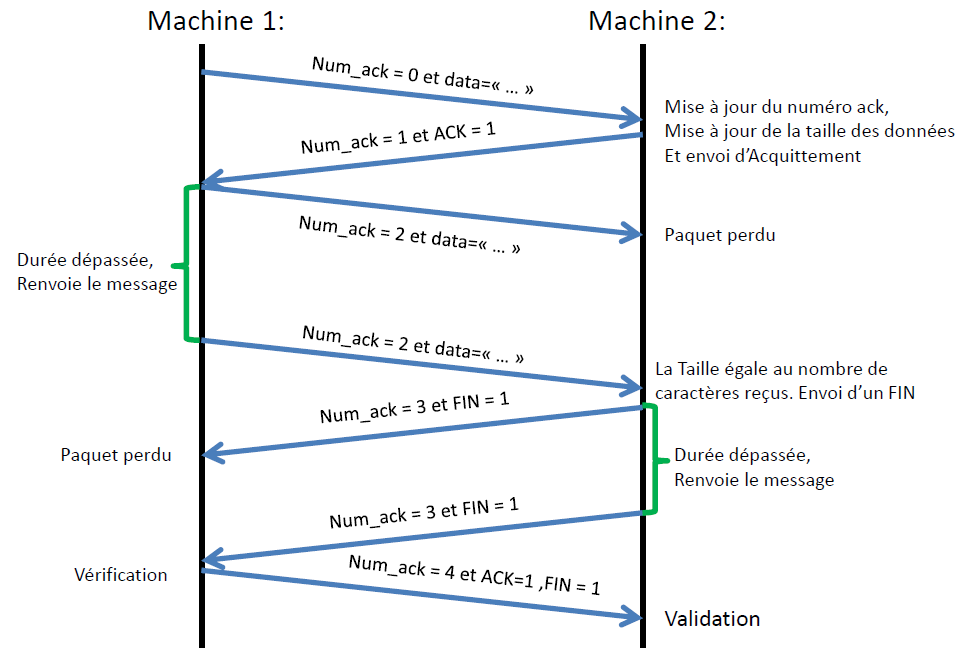
\includegraphics[scale=0.6]{protocoleReseau}
\end{center}

\bigskip


Les longs messages dépassant la taille d’une trame sont gérés par
un séquencement et l’ajout d'une taille totale dans l’en-tête de la classe MailHeader. \\


Les messages sont vérifiés grâce à leur numéro d'acquittement et par leur type ACK, FIN ou donnée, ceci dans le but de conserver l'ordre des messages et d'assurer une commmunication cohérente entre le récepteur et l'émetteur.
\newpage

\section{Extensions des fonctionnalités}

D'autres fonctionnalités ont été étudiées et/ou implémentées mais ne sont pas fonctionnelles à ce jour.
Parmi ces fonctionnalités on compte :
\bigskip
\begin{itemize}\renewcommand{\labelitemi}{$\bullet$}
\item L'ajout de l'option -mv (nom)(rep) servant à déplacer un fichier ou un répertoire de nom \textit{nom} vers le répertoire \textit{rep}.\bigskip
\item L'extension de l'option -cp (nom1) (nom2) pour qu'elle permette d'effectuer une copie d'un fichier \textit{nom1} présent dans le système vers un nouveau fichier \textit{nom2} également dans le système.\bigskip
\item L'augmentation de la taille maximale des fichiers à 120ko, qui pourrait être réalisée en utilisant une classe similaire à FileHeader mais permettant le stockage de 32 entiers (soit 128 octets) au lieu de 30 actuellement.\bigskip
\item L'extension des commandes mkdir et rmdir afin de permettre l'utilisation de chemins (exemple : mkdir dir1/dir2/newdir).\bigskip
\item La gestion des fichiers ouverts à l'aide d'un tableau défini au niveau du système.\bigskip
\item La gestion concurrente de plusieurs threads accédant au système du fichiers. Ceci nécessiterait que chaque thread possède sa propre table des fichiers ouverts en plus de celle définie pour le système, ce qui permettrait le blocage des commandes interdites comme la modification ou la fermeture d'un fichier ouvert par thread différent du thread courant.\bigskip
\item Dans la partie réseau, l'adaptation du délai avant réémission des messages perdus à l'environnement. Notamment, la valeur du timer utilisé pourrait être calculée en fonction du débit dont bénéficie la machine sur le réseau.
\end{itemize}




\chapter{Tests utilisateur}

\section{Entrées/Sorties}

\textbf{testEtape2.c :} Programme mettant en place l'interaction avec l'utilisateur via les E/S standards. Ce programme utilise les appels système GetChar, PutChar, GetString, PutString, GetInt et PutInt. Comme détaillé dans les spécifications, si GetChar reçoit une chaîne de caractères, seul le premier caractère de la chaîne est stocké. Le prochain appel à GetString affiche alors le reste des caractères, ce qui montre un mauvais comportement. L'utilisateur doit donc entrer strictement un caractère lors de l'appel à GetChar.
\bigskip

\section{Threads utilisateur}

\textbf{makethreads.c :}
Crée 6 threads et leur demande d’afficher chacun un caractère qui sera aussi affiché par le thread principal. Le thread principal
affiche un caractère puis attend chaque thread alternativement. Ce test permet de vérifier que les
threads se lancent, exécutent une fonction et sont bien attendus par le main en cas d'appel à Join.\\

\textbf{test3\_threads.c :} Crée deux threads affichant l’entier 44, le caractère ‘\_’ puis 5 ou 10 en
fonction du thread 1 ou 2. Ce test permet de vérifier que l’on peut récupérer les informations
concernant le thread et le non dépassement de pile.\\

\textbf{test3\_1threads.c :} Crée des threads qui affichent chacun une valeur différente t[i] d’un
tableau t suivie d’un retour à la ligne. Le thread principal fait ensuite un Join() pour tous les threads
créés. Ce test simple permet de vérifier la validité du fonctionnement de UserThreadCreate(), sa
valeur de retour, et UserThreadJoin().
\newpage

\textbf{testMultithreading.c :} Crée un grand nombre de threads afin de vérifier le nombre de threads maximal supporté. Notre système d'exploitation pouvant supporter au plus 16 threads par processus, le système bloque à la création d'un thread supplémentaire en raison d'un dépassement de capacité mémoire.\\

\textbf{testSemThreads.c :} Crée un producteur et 3 consommateurs. Le producteur initialise un buffer avec une suite de caractères ASCII puis signale aux consommateurs qui attendent que le buffer est plein. Le consommateur doit remplacer le caratère lu du buffer avec un caractère 'x' pour indiquer aux autres consommateurs que le caratère a été lu. Ce test permet de tester la bonne utilisation des sémaphores au niveau utilisateur.
\bigskip

\section{Processus}

\textbf{testForkExec.c:} Crée seul processus monothreadé.
\bigskip

\textbf{testForkExec1.c:} Crée un seul processus multithreadé.
\bigskip

\textbf{testForkExec2.c:} Crée un processus monothreadé et un processus multithreadé.
\bigskip

\textbf{testForkExec3.c:} Crée deux processus multithreadés avec un affichage.
\bigskip

\textbf{testForkExec4.c:} Crée deux processus multithreadés gérés avec des entrées/sorties.
\bigskip

\section{Système de fichiers}

Les commandes disponibles peuvent être testées directement dans le système de fichiers.


\section{Réseau}

\textbf{nettest.cc:} Teste le fonctionnement client/serveur. Effectue notamment un test simple d'envoi et de réception des données ainsi qu'un test en anneau incluant 3 machines.
\bigskip



\chapter{Organisation du travail en équipe}
Au cours du projet, chacun a contribué à plusieurs parties afin d'avancer autant que possible tout en comprenant
comment fonctionnent les différentes fonctionnalités de NachOS. L'intégration a été faite au fur et à mesure du développement des différents éléments. La première partie du projet sur les entrées/sorties a été développée en commun afin que tout le groupe acquière une bonne compréhension du système de base. Le travail a ensuite été réparti comme suit :
\bigskip


\textbf{Mohd Thaqif ABDULLAH HASIM :}

Entrées/Sorties : Implémentation, tests\\
Threads : Debug\\
Processus : Debug\\
Réseau : Conception, implémentation, tests
\bigskip 
 
\textbf{Florian BARROIS:}

Entrées/Sorties : Tests\\
Threads : Conception, implémentation, tests, debug\\
Processus : Conception, tests, debug\\
Système de fichiers : Conception, implémentation\\
Rédaction du rapport
\bigskip 

\textbf{Hosseim NAHAL:}

Threads : Conception, implémentation, debug\\
Système de fichiers : Conception, implémentation, tests, debug
\bigskip

\textbf{Cédric GARCIA:}

Entrées/Sorties : Conception, implémentation\\
Threads : Conception, implémentation, tests, debug\\
Processus : Conception, implémentation, tests, debug\\
Réseau : Conception, implémentation, tests, debug
\bigskip

\textbf{Peio RIGAUX:}

Entrées/Sorties : Debug, tests\\
Processus : Tests\\
Réseau : Conception, implémentation\\
Contribution au rapport




\chapter{Retour global sur le projet}

\`A la fin de la période de projet, notre système possède au moins une implémentation basique de chaque étape demandée. La rigueur du groupe lors du développement a permis d'intégrer facilement toutes les facettes du système entre elles et favorise la reprise du projet pour d'éventuelles améliorations futures.
\bigskip

Malgré une gestion du temps et la communication au sein du groupe qui auraient pu être améliorées, le système présente la plupart des fonctionnalités de base qu'un utilisateur peut attendre de nos jours.
\bigskip

De manière générale, la diversité des parties d'un système que nous avions à implémenter nous a apporté une meilleure compréhension des systèmes d'exploitation et nous a permis d'améliorer nos qualité de développement bas niveau.




\end{document}